\documentclass[letterpaper]{article}
\usepackage[utf8]{inputenc}
\usepackage[T1]{fontenc}
\usepackage{microtype}
\usepackage{amsmath,amssymb,amsfonts}
\usepackage{graphicx}
\usepackage{booktabs}
\usepackage{xcolor}
\usepackage[numbers]{natbib}
\usepackage{hyperref}
\usepackage[margin=1in]{geometry}
\graphicspath{{figures/}}

\title{The Limits of Test-Time Compute in Iterative Denoisers:\\
A Depth Law, and Two Things It Does \emph{Not} Buy}
\author{Hafez Al-Khatib \\ American University of Beirut}
\date{}

\begin{document}
\maketitle

\begin{abstract}
Spending more computation at inference is widely assumed to help. For iterative denoisers---energy-based
models, score networks, and diffusion---we make this precise and, more importantly, bound it. First, the
optimal number of refinement steps follows a power law $K^{*}(\sigma)=C\sigma^{\alpha}$ in the noise level.
Under a matched protocol the exponent is strikingly stable ($\alpha=1.370\pm0.010$ over $25$ runs; an
$F$-test cannot distinguish architectures, $F=0.79$), the form survives a $3000\times$ range of model size
($R^2>0.98$), and one calibration point predicts the whole curve to $7.5\%$ mean error. But $\alpha$ is
\emph{regime-scoped}, not universal: changing architecture and training recipe shifts it to $1.27$. The law
is also \emph{corruption-conditioned}---it holds for stochastic corruptions (Gaussian, speckle, Poisson;
$R^2>0.95$) but breaks for deterministic ones (blur, JPEG), delimiting when test-time compute helps at all.
Second, and against intuition, we show two hard limits of this compute. \textbf{(i)} It buys no \emph{per-instance}
adaptivity: at a fixed noise level the optimal depth varies by only $\sim\!0.6$ steps across inputs, so
there is nothing to allocate. \textbf{(ii)} It is information-\emph{dissipative}: each refinement step
\emph{destroys} distributional information about the input---far-OOD detectability decays monotonically
with depth (AUROC $0.92\!\to\!0.77$), while near-OOD detectability sits at chance at every depth---so the
\emph{pre}-refinement energy is the better anomaly score.
We ground both the law and its limits in classical iterative-regularization theory. The practical message is
two-sided: a one-line rule sets the compute budget, and two tempting uses of that compute are
unavailable.
\end{abstract}

\section{Introduction}
The dominant story in inference-time scaling is optimistic: let the model ``think longer'' and it does
better---in language reasoning \citep{snell2024}, in energy-based transformers \citep{gladstone2025}, in
diffusion refinement. Iterative denoisers are the cleanest place to study this claim quantitatively: an
energy-based model runs gradient descent on a learned energy $E_\theta(\mathbf{x})$, and additional steps
$K$ can improve or, past a point, degrade the estimate.

We give the operational law \emph{and} its boundary. Our contributions:
\begin{enumerate}
\item \textbf{A calibrated depth law.} $K^{*}(\sigma)=C\sigma^{\alpha}$ holds with $R^2>0.98$ across
datasets, architectures, and $3000\times$ in scale. The exponent is tightly $1.37$ \emph{within} a matched
regime but regime-scoped across recipes; one measurement calibrates the curve (Sec.~4).
\item \textbf{Iteration, not architecture.} A feedforward denoiser is exactly flat in $K$: the capability
is intrinsic to iterating a gradient field (Sec.~5).
\item \textbf{A phase boundary.} The law is corruption-conditioned---it holds for stochastic corruptions and
breaks for deterministic ones ($K^{*}\!\approx\!0$), delimiting when test-time compute helps at all (Sec.~6).
\item \textbf{Two negative results.} Test-time compute here yields \emph{no} per-instance adaptivity
(Sec.~6.1), and it \emph{destroys} distributional information rather than sharpening it (Sec.~6.2). Both
correct natural hypotheses and both are, we argue, the more useful part of the paper.
\end{enumerate}
We deliberately foreground the limits: the positive law is close to classical early-stopping theory, whereas
the boundary---what ``thinking longer'' cannot do for an iterative denoiser---is less appreciated.

\section{Related Work}
\paragraph{Iterative regularization.} Early-stopped gradient descent is a spectral filter whose optimal
stopping time scales as a power law in the noise \citep{landweber1951,yao2007,raskutti2014}; our law is the
expected form. We contribute its systematic measurement for neural denoisers, its scale/architecture
robustness with statistics, a calibration rule, and its limits.
\paragraph{Iterative denoisers.} EBMs \citep{lecun2006,du2019}, score matching \citep{song2019}, and
diffusion \citep{ho2020,song2021} share a gradient-refinement operator, explaining why one law spans them.
\paragraph{Test-time compute, verification, OOD.} Inference-time scaling \citep{snell2024} and energy-based
``thinking'' \citep{gladstone2025} motivate the compute-helps view we bound here. Energy is a common OOD
score \citep{liu2020,grathwohl2020}; our Sec.~6.2 characterizes how that signal behaves \emph{under}
refinement, complementing reconstruction-based diffusion OOD detection, which exploits the same erasure
(``healing'') of anomalies \citep{graham2023}.

\section{Setup}
Given clean $\mathbf{x}$ and noise level $\sigma$, form $\mathbf{u}_0=\mathbf{x}+\sigma\epsilon$ and iterate
$\mathbf{u}_{k+1}=\mathbf{u}_k-\eta_k\nabla E_\theta(\mathbf{u}_k)$ with a decaying step size. Models are
trained by denoising score matching. Per image, $K^{*}=\arg\max_k\mathrm{PSNR}(\mathbf{u}_k,\mathbf{x})$; we
average over held-out data and fit $\log K^{*}=\log C+\alpha\log\sigma$. Unless noted, results use
$2$--$3$ seeds per configuration; we report means with standard deviations and, where stated, bootstrap
$95\%$ confidence intervals.

\section{A Calibrated Depth Law}
\paragraph{Within-regime stability.} Over $25$ matched runs spanning four datasets and five architectures,
$\alpha=1.370\pm0.010$ (Fig.~\ref{fig:law}). Per dataset: CIFAR-10 $1.376\pm0.004$, Fashion-MNIST $1.372\pm0.005$, MNIST
$1.356\pm0.009$. Across CIFAR architectures the values are indistinguishable (KAN $1.376$, GELU $1.378$,
SiLU $1.379$, Tanh $1.373$); an $F$-test for between- vs.\ within-architecture variance gives $F=0.79<1$,
i.e., we cannot reject architecture-independence. A bootstrap over runs gives $\alpha=1.377$, $R^2=0.981$,
$95\%$ CI $[1.23,1.60]$.
\begin{figure}[t]\centering
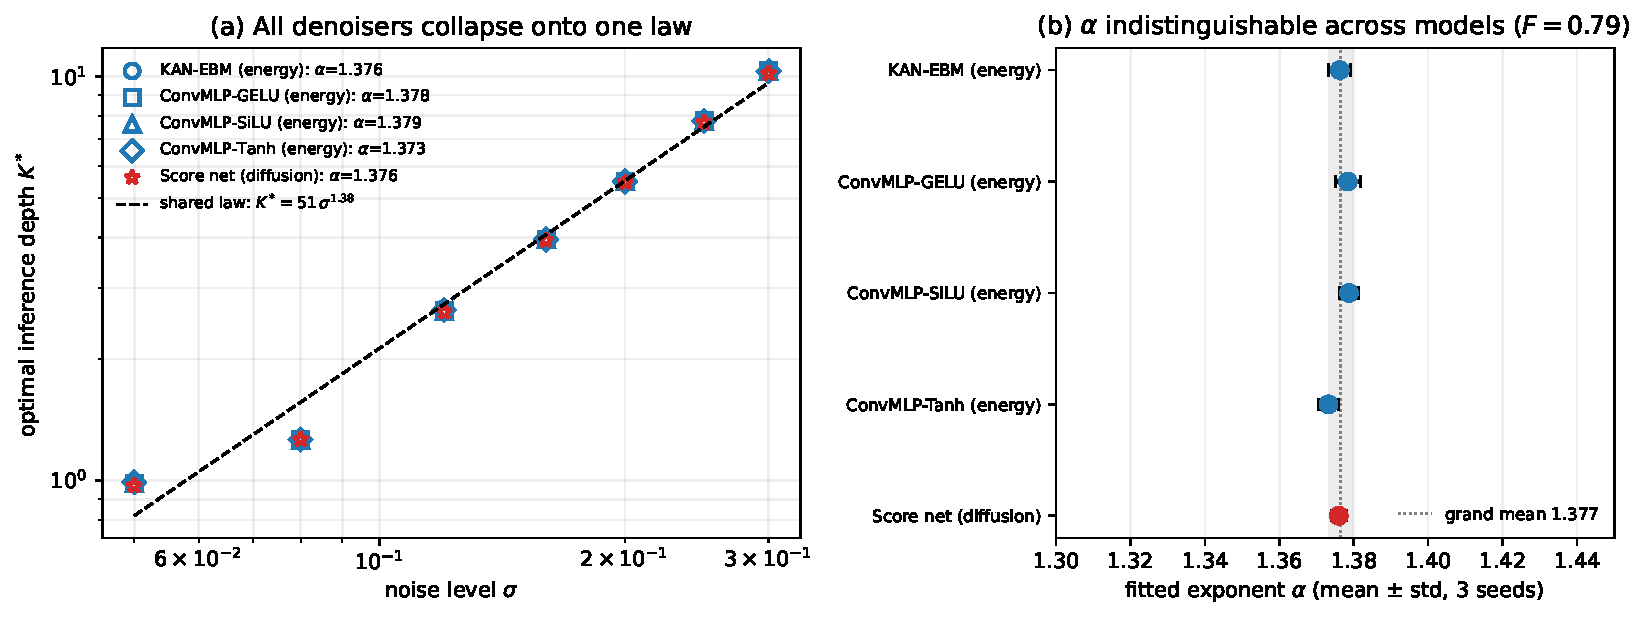
\includegraphics[width=\linewidth]{fig_universality}
\caption{The depth law. (a) $K^{*}(\sigma)$ for four energy-based architectures and a score network
collapse onto one power law. (b) Fitted exponents are statistically indistinguishable across models
($F=0.79$); shaded band is $\pm 1$ std around the grand mean.}
\label{fig:law}
\end{figure}
\paragraph{Scale robustness, regime-scoped exponent.} Table~\ref{tab:scale} extends the law over a
$3000\times$ range of model size. The \emph{form} is intact ($R^2>0.98$); the \emph{exponent} shifts to
$1.27$ for a globally-pooled energy trained on mixed noise, showing $\alpha$ is a property of the
operator's spectrum and recipe, not a universal constant.
\begin{table}[h]\centering
\begin{tabular}{lrcc}
\toprule
Model & Params & $\alpha$ & $R^2$ \\
\midrule
Local KAN-EBM (matched regime) & $3.2\!\times\!10^{4}$ & $1.369$ & $0.989$ \\
Global Conv-EBM (mixed-$\sigma$) & $2.4\!\times\!10^{6}$ & $1.267$ & $0.997$ \\
Pretrained DDPM score net & $\sim\!10^{8}$ & $1.366$ & $0.994$ \\
\bottomrule
\end{tabular}
\caption{Form scale-robust; exponent regime-scoped ($1.27$--$1.37$).}
\label{tab:scale}
\end{table}
\paragraph{One-shot calibration.} Fixing $\alpha=1.37$ and estimating $C$ from a single $\sigma=0.16$
predicts $K^{*}$ across the range with $7.5\%$ mean and $25\%$ worst-case error over $26$ runs---matching a
full seven-point fit while removing the sweep.

\section{Iteration, Not Architecture}
At $\sigma=0.2$, a feedforward denoiser trained with the same objective is exactly flat: $25.29$\,dB at every
$K$, having no gradient field to iterate. The EBM shows semiconvergence: PSNR rises to $25.9$\,dB near
$K=5$, then decays to $18.7$\,dB by $K=50$ as over-denoising erases signal (Fig.~\ref{fig:semiconv}). The
capacity to convert compute into quality is thus a property of the iterative operator, not the
parameterization.
\begin{figure}[t]\centering
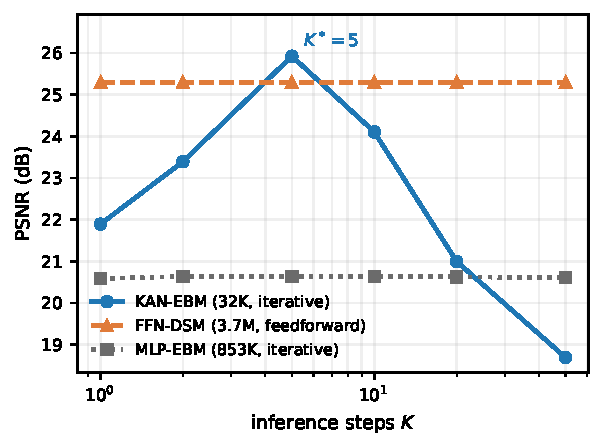
\includegraphics[width=0.62\linewidth]{fig_semiconvergence}
\caption{Semiconvergence vs.\ flatness (CIFAR-10, $\sigma=0.2$). The energy model converts steps into
quality and then over-denoises; the feedforward baseline is exactly flat in $K$; a poorly conditioned
iterative model is flat at a lower level. The $K$-dial exists only for iterative operators.}
\label{fig:semiconv}
\end{figure}

\section{A Phase Boundary: Which Corruptions Admit Test-Time Compute}
The law presupposes that iteration helps at all---and it does not always. Sweeping five corruption types
across three architectures (Table~\ref{tab:phase}, Fig.~\ref{fig:phase}), we find a clean dichotomy. For \emph{stochastic},
signal-independent corruptions---additive Gaussian, speckle, and Poisson noise---the depth law holds with
$R^{2}\in[0.95,0.99]$ and $K^{*}$ grows with severity. For \emph{deterministic} degradations---Gaussian
blur and JPEG compression---it breaks: the optimal depth is $K^{*}\!\approx\!0$ (a single step is best, or
iteration never helps) and no power law fits ($R^{2}\le0.31$). The boundary follows from the theory: energy
descent removes an additive residual, and a deterministic operator leaves none to remove. Test-time compute
for an iterative denoiser is thus \emph{corruption-conditioned}: useful for stochastic inverse problems,
inert for deterministic ones---a concrete guide to when ``thinking longer'' can help at all.
\begin{table}[h]\centering
\begin{tabular}{lccc}
\toprule
Corruption & Type & Verdict & $R^{2}$ (range) \\
\midrule
Gaussian & stochastic & \textbf{law} & $0.95$--$0.99$ \\
Speckle & stochastic & \textbf{law} & $0.98$--$0.98$ \\
Poisson & stochastic & \textbf{law} & $0.97$--$0.99$ \\
Blur & deterministic & breaks & $\approx0$ ($K^{*}{=}0$) \\
JPEG & deterministic & breaks & $\le0.31$ \\
\bottomrule
\end{tabular}
\caption{The depth law holds for stochastic corruptions and breaks for deterministic ones, consistently
across three architectures (KAN-, GELU-EBM, U-Net).}
\label{tab:phase}
\end{table}
\begin{figure}[t]\centering
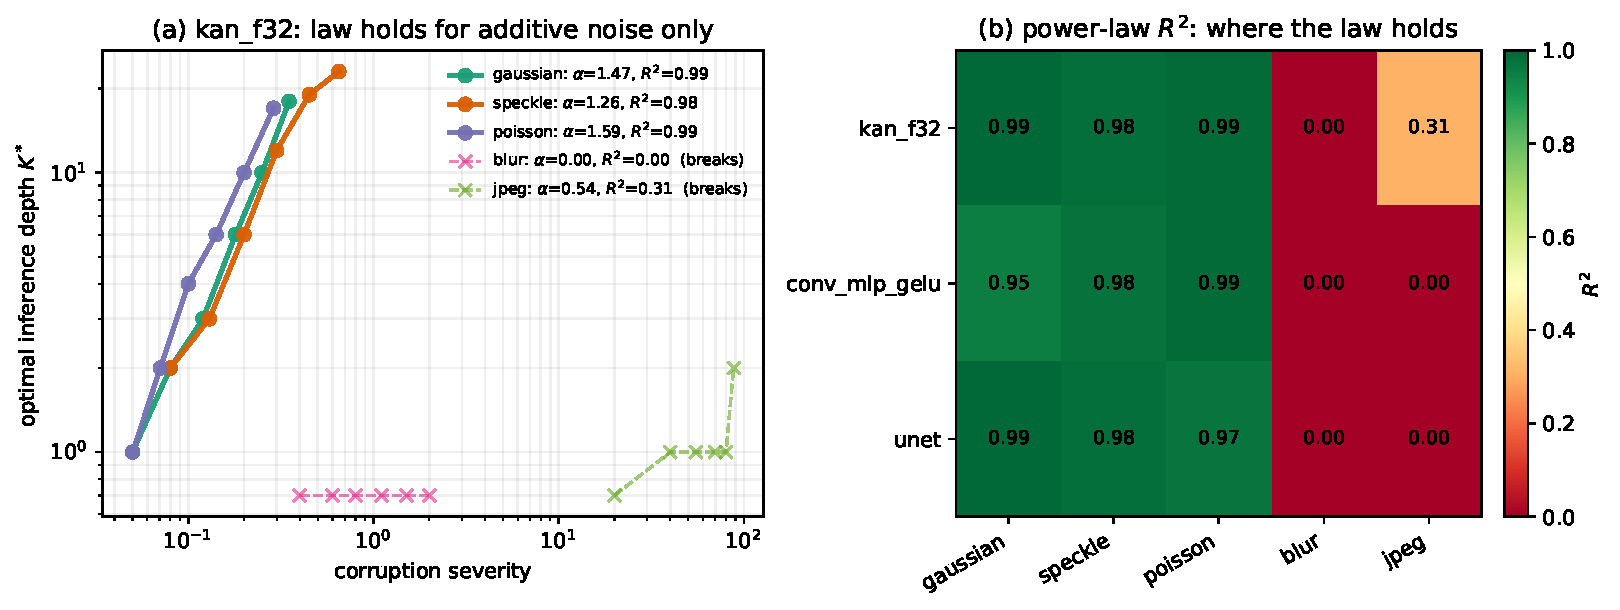
\includegraphics[width=\linewidth]{fig_phase_diagram}
\caption{The phase boundary. (a) $K^{*}$ grows with severity under a power law for stochastic corruptions
but not for deterministic ones. (b) Power-law $R^{2}$ across corruptions $\times$ architectures: the
law/breaks dichotomy is architecture-consistent.}
\label{fig:phase}
\end{figure}

%% ===== TASK9-FRONTIER-SCAFFOLD (uncomment + fill when remote frontier data returns) =====
%% Fill every \NUM{...} from outputs/inference_frontier/frontier.json /
%% outputs/group_kan/fine_grid_group_kan_32k.json; KEEP EXACTLY ONE framing
%% paragraph (pre-registered verdict from exp_inference_frontier.py --analyze);
%% copy outputs/inference_frontier/frontier.png -> figures/frontier.png.
%
%\section{The Inference Frontier: Trading Head Capacity for Depth}
%\label{sec:frontier}
%The depth law fixes how quality scales with iteration count for a given
%energy head. A deployment question remains: at a \emph{fixed inference FLOP
%budget}, should one spend the budget on a heavier head taking fewer descent
%steps, or a lighter head taking more? We measure this directly. For each
%head we count the FLOPs of one descent step (one energy forward plus the
%input-gradient backward; matmul/conv operations, counted with PyTorch's
%\texttt{FlopCounterMode}) and record PSNR after every step
%($K{=}0{\dots}30$, five noise levels, 500 CIFAR-10 test images, two noise
%seeds), yielding quality-versus-cumulative-FLOPs curves. The comparison
%criterion was pre-registered before data collection: the lighter head must
%lead by ${\geq}0.3$\,dB over a contiguous budget range in at least three of
%five noise levels and both seeds, with the parameter-matched pair
%KAN-32K/KAN-110K primary.
%
%% --- PASS framing (delete if verdict=FAIL) ---
%Depth substitutes for capacity. The 32K-parameter head, given its FLOP
%budget in extra steps, matches or exceeds the 110K head by
%$\NUM{X.X}$--$\NUM{X.X}$\,dB across budgets of
%$\NUM{X}$--$\NUM{X}$\,MFLOPs/image (Fig.~\ref{fig:frontier}), and a grouped
%KAN head~\citep{yang2025kat} at $8.3$K parameters extends the frontier
%further. The depth law of Sec.~4 then tells the practitioner how many steps
%that budget should buy at each noise level: the two results compose into a
%calibration-free deployment rule.
%
%% --- FAIL framing (delete if verdict=PASS) ---
%Depth does \emph{not} substitute for capacity. At every matched budget the
%heavier head dominates (max lighter-head advantage
%$\NUM{X.X}$\,dB $<$ the pre-registered $0.3$\,dB margin;
%Fig.~\ref{fig:frontier}). Together with the absence of per-instance
%adaptivity and the dissipative character of refinement (Sec.~7), this adds a
%third boundary: iteration buys accuracy only along the noise axis of the
%depth law, not as a substitute for model capacity at inference time.
%
%\begin{figure}[t]\centering
%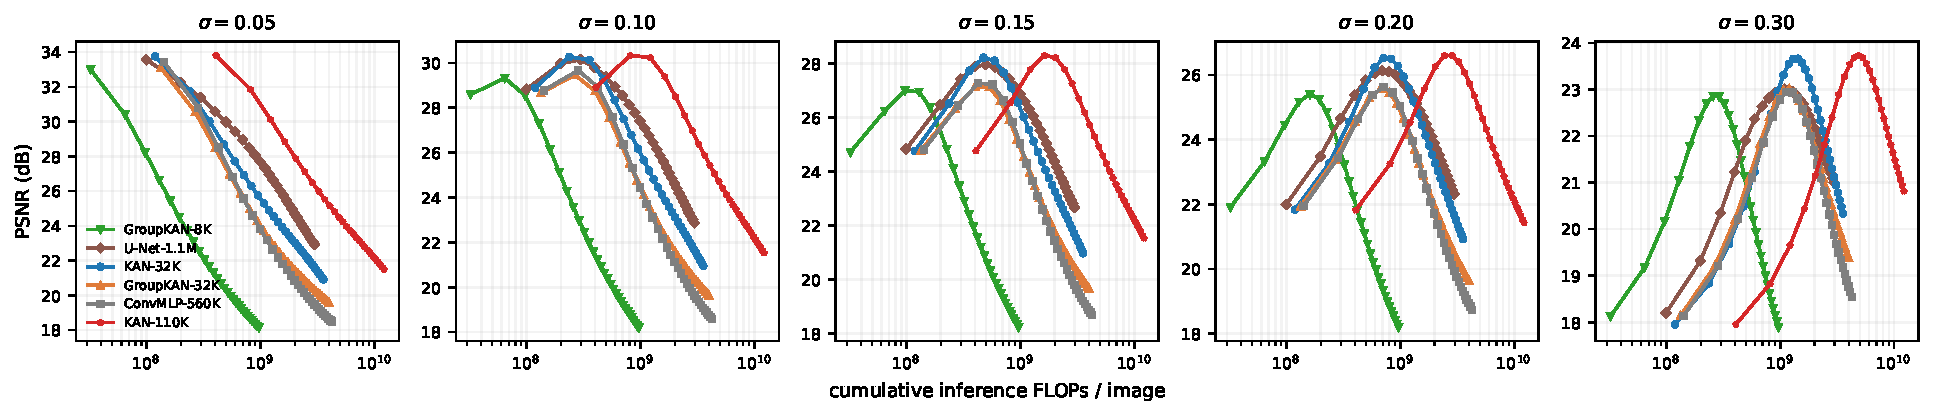
\includegraphics[width=\linewidth]{frontier}
%\caption{Quality vs.\ cumulative inference FLOPs per image (log axis), one
%panel per noise level, one curve per energy head; markers are descent steps.
%The pre-registered comparison is KAN-32K vs.\ KAN-110K.}
%\label{fig:frontier}
%\end{figure}
%
%A sixth architecture on the depth law: the grouped KAN head trained under
%the identical denoising-score-matching recipe follows
%$K^{*}(\sigma)=C\sigma^{\alpha}$ with $\alpha=\NUM{X.XXX}$
%($R^2=\NUM{0.XXX}$, 95\% CI $[\NUM{X.XX},\NUM{X.XX}]$), consistent with the
%iteration-not-architecture finding. [Only if R^2>0.95 quality gate passes;
%F=0.79 remains attributed to the original five architectures.]
%% ===== END TASK9-FRONTIER-SCAFFOLD =====

\section{Two Things Test-Time Compute Does Not Buy}
\subsection{No per-instance adaptive depth}
If $K^{*}$ varied enough across inputs, one could budget compute per image. It does not: at fixed $\sigma$,
the per-image $K^{*}$ has standard deviation $\sim\!0.6$ steps (range $3$--$6$). Almost all the signal is the
across-$\sigma$ law; a per-instance controller matches the calibrated rule to within noise. Adaptive
inference-depth allocation, at least for denoising, is not where the leverage is.

\subsection{Refinement is information-dissipative}
It is natural to expect the energy \emph{after} refinement to be a sharper confidence/OOD signal than the raw
input energy. The reverse is true. At a matched, deployable descent depth, OOD detectability
(AUROC, CIFAR-10 vs.\ SVHN) falls \emph{monotonically} with $K$: $0.92$ at $K=0$ (static energy) $\to 0.77$
at $K=30$; for semantically near OOD (CIFAR-100) it sits at chance ($0.51$--$0.53$) at all depths
(Fig.~\ref{fig:ood}).
\begin{figure}[t]\centering
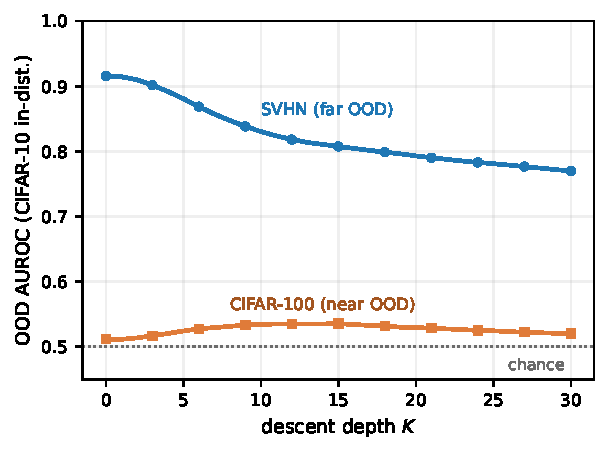
\includegraphics[width=0.62\linewidth]{fig_ood_decay}
\caption{Refinement is information-dissipative. Far-OOD detectability by the energy decays monotonically
with descent depth; near-OOD detectability is at chance at every depth. The best anomaly score is the
energy \emph{before} refinement.}
\label{fig:ood}
\end{figure} Gradient
descent is dissipative---it contracts phase-space volume and pulls every input, including OOD inputs, toward
the learned manifold, erasing the distributional signal. The \emph{pre}-refinement energy is therefore the
better anomaly score. This both explains and unifies with reconstruction-based diffusion OOD, which succeeds
by measuring exactly this erasure \citep{graham2023}. Practically: if an iterative model must flag anomalies,
score them \emph{before} it thinks, not after.

\section{Practical Takeaways}
(1) To set inference depth, measure $K^{*}$ at one noise level and apply $K^{*}(\sigma)=C\sigma^{1.37}$;
re-fit $\alpha$ if the architecture/recipe changes. (2) Do not over-refine---quality peaks early and decays.
(3) Do not expect per-image compute budgeting or post-refinement confidence from an iterative denoiser; use
the input energy for OOD and the calibrated rule for compute.

\section{Discussion: Inference Depth as Compute Allocation}
Our results are, at heart, statements about the \emph{value of computation}. $K^{*}(\sigma)$ is the
compute-optimal stopping point; the rise-then-decay of quality is the denoising analogue of the
\emph{over-thinking} now widely reported for reasoning models, where accuracy first improves and then
degrades with additional inference \citep{snell2024}. Our phase boundary sharpens this into a
value-of-computation criterion: iteration is worth spending only for stochastic corruptions and is inert
for deterministic ones---a structural predictor of \emph{when} thinking longer can help at all. This
connects the denoising setting to the broader effort to allocate test-time compute rationally, from
cost-aware ``rational metareasoning'' for language models \citep{ram2024} to energy-minimization views of
reasoning where the energy itself supplies a termination criterion \citep{du2022}. It also echoes a
normative principle from cognitive science and neuroscience---that agents allocate limited computational
(indeed metabolic) resources against their expected value \citep{lieder2020,christie2015}. We do not claim
a normative derivation here; rather, our empirical law, its calibration, and its corruption-conditioned
boundary supply concrete, measured constraints that such a theory of optimal inference-time compute would
need to reproduce.

\section{Limitations}
``Universal'' describes the law's form, not its exponent. The study is confined to additive-noise denoising
at low resolution; the largest model is probed, not trained under our protocol; and the dissipation result
concerns energy-based/reconstruction inference specifically. We make no claim that energy descent provides
adaptive compute or calibrated confidence; we show it does not, here.

\section{Conclusion}
Iterative denoisers obey a simple, scale-robust, calibratable depth law with a regime-scoped exponent, and
the capability is intrinsic to iteration. Its boundary is equally concrete: test-time energy descent buys no
per-instance adaptivity and erases the distributional information it is often assumed to preserve. Both the
rule and its limits should help practitioners decide how long to let an iterative model think---and when not
to bother.

\paragraph{Reproducibility.} Protocol, seeds, fitting code, and the scripts producing every number and figure
are released; all results use held-out data and reported seeds.

\begin{thebibliography}{99}
\small
\bibitem{landweber1951} L. Landweber. An iteration formula for Fredholm integral equations. \emph{Amer. J. Math.}, 1951.
\bibitem{yao2007} Y. Yao, L. Rosasco, A. Caponnetto. On early stopping in gradient descent learning. \emph{Constr. Approx.}, 2007.
\bibitem{raskutti2014} G. Raskutti, M. Wainwright, B. Yu. Early stopping and non-parametric regression. \emph{JMLR}, 2014.
\bibitem{lecun2006} Y. LeCun et al. A tutorial on energy-based learning. \emph{Predicting Structured Data}, 2006.
\bibitem{du2019} Y. Du, I. Mordatch. Implicit generation and generalization with energy-based models. \emph{NeurIPS}, 2019.
\bibitem{song2019} Y. Song, S. Ermon. Generative modeling by estimating gradients of the data distribution. \emph{NeurIPS}, 2019.
\bibitem{ho2020} J. Ho, A. Jain, P. Abbeel. Denoising diffusion probabilistic models. \emph{NeurIPS}, 2020.
\bibitem{song2021} Y. Song et al. Score-based generative modeling through SDEs. \emph{ICLR}, 2021.
\bibitem{snell2024} C. Snell et al. Scaling LLM test-time compute optimally. \emph{arXiv:2408.03314}, 2024.
\bibitem{gladstone2025} A. Gladstone et al. Energy-based transformers are scalable learners and thinkers. \emph{arXiv:2507.02092}, 2025.
\bibitem{liu2020} W. Liu et al. Energy-based out-of-distribution detection. \emph{NeurIPS}, 2020.
\bibitem{grathwohl2020} W. Grathwohl et al. Your classifier is secretly an energy based model. \emph{ICLR}, 2020.
\bibitem{graham2023} M. Graham et al. Denoising diffusion models for out-of-distribution detection. \emph{CVPR-W}, 2023.
\bibitem{ram2024} C.~N. De~Sabbata, T.~R. Sumers, B.~AlKhamissi, A.~Bosselut, T.~L. Griffiths. Rational metareasoning for large language models. \emph{arXiv:2410.05563}, 2024.
\bibitem{du2022} Y. Du, S. Li, J. Tenenbaum, I. Mordatch. Learning iterative reasoning through energy minimization. \emph{ICML}, 2022.
\bibitem{yang2025kat} X. Yang, X. Wang. Kolmogorov--Arnold transformer. \emph{ICLR}, 2025.
\bibitem{lieder2020} F. Lieder, T. Griffiths. Resource-rational analysis: understanding human cognition as the optimal use of limited computational resources. \emph{Behavioral and Brain Sciences}, 2020.
\bibitem{christie2015} S.~T. Christie, P. Schrater. Cognitive cost as dynamic allocation of energetic resources. \emph{Frontiers in Neuroscience}, 9:289, 2015.
\end{thebibliography}
\end{document}
